\documentclass[sigconf,nonacm]{acmart}

\setcopyright{none}
\settopmatter{printacmref=false,printfolios=true}


% --- Packages ---
\usepackage[utf8]{inputenc}
\usepackage{graphicx}
\usepackage{amsmath, amsthm}
\usepackage{booktabs}

% --- Build switches ---
\newif\iffinalresults
% Set to \finalresultstrue for submission once real-data runs are available.
\finalresultstrue

% --- Writing-time placeholders (auto-populated before submission) ---
\newcommand{\autofill}{\textit{(auto-populated)}}
\usepackage{caption}
\usepackage{subcaption}
\usepackage{xcolor}
\usepackage{hyperref}
% Cross-references (e.g., \Cref{fig:...}); load after hyperref.
\usepackage[nameinlink]{cleveref}
\usepackage{tabularx}
\usepackage{multirow}
\usepackage{enumitem}
\usepackage{float}
\usepackage{algorithm}
\usepackage{algpseudocode}
\usepackage{pifont}
\newcommand{\cmark}{\ding{51}}

% --- Custom commands ---
\newcommand{\compa}{\textsc{Compass}}
\newcommand{\ecl}{\textsc{ECL}}
\newcommand{\mas}{\textsc{MAS}}
\newcommand{\decol}{\textsc{DÉCOL}}
\newcommand{\scores}{s}
\newcommand{\params}{\theta}
\newcommand{\fairnessgap}{\Delta_{\mathrm{EOpp@K}}}
\newcommand{\entropy}{H}
\newcommand{\coverage}{C}
\newcommand{\lagrangian}{\mathcal{L}}

\newtheorem{theorem}{Theorem}
\newtheorem{lemma}{Lemma}

% Metadata hooks (reproducibility, runs)
% Auto-populated run metadata from outputs.zip
\newcommand{\OULADRunID}{\detokenize{oulad_run_v1_oulad_v1_seed42_20260126T031033Z_LOCAL}}
\newcommand{\ASSISTRunID}{\detokenize{assistments_run_v1_assistments_2009_2010_v1_seed42_20260126T031036Z_LOCAL}}
\newcommand{\SYNTHRunID}{\detokenize{synthetic_run_v1_synthetic_v1_seed42_20260126T234652Z_LOCAL}}

\newcommand{\OULADPolicyHash}{6acd976bcc40e301aa66da4db0b79a1e60922047f26079e775a803a763c295b6}
\newcommand{\ASSISTPolicyHash}{a04865e9097172a9a5ed53e386eb4d7d270e22e0f9ae57bea8739ae449d5cbb8}
\newcommand{\SYNTHPolicyHash}{0b0abb0ab926023d8f98a6eba3f59fae05e95d0c4a2d8585f38f791deef94cf0}

\newcommand{\CompassRepoURL}{\url{https://github.com/rtales/compass-contestable-governance-artifacts}}

\newcommand{\SYNTHRecipePath}{configs/recipes/synthetic.yaml}

\newcommand{\SYNTHRecipeHash}{e53c4ed010bff83ca8a8a147ae199e97e23d80c5df846e58b7d5744786e72664}

\newcommand{\SYNTHDatasetManifestHash}{01e6c15b986c94a65d77d8b7b62c01b4863b2e53a37b121e13683f1075b17765}

\newcommand{\SYNTHModelHash}{20b36e5c7d1bebb4ba1dca847ec91b222f20c69ff1c8b6a9dd19bb645c902bf5}

\newcommand{\SYNTHSeed}{42}

\newcommand{\SYNTHCreatedUTC}{20260126T234652Z}

\newcommand{\SYNTHContestScore}{4/4}

\newcommand{\SYNTHReplayable}{true}

% Numeric result macros (filled for submission)
% Auto-populated from outputs.zip (artifact bundle).
\newcommand{\OULADN}{6519}
\newcommand{\OULADPrev}{0.466}
\newcommand{\ASSISTN}{105107}
\newcommand{\ASSISTPrev}{0.683}
\newcommand{\SYNTHN}{1000}
\newcommand{\SYNTHPrev}{0.445}
\newcommand{\EoppMax}{0.05}


\emergencystretch=3em
\tolerance=2500
\begin{document}

\title{Governing by Artifacts: An Auditable Constraint-Based Framework for Contestable Educational Decision Systems}

\author{Tales Matos}
\affiliation{%
  \institution{Federal University of Cear\'a}
  \department{Department of Computer Science}
  \country{Brazil}}
\email{tales.matos@dc.ufc.br}

\author{Jose Macedo}
\affiliation{%
  \institution{Federal University of Cear\'a}
  \department{Department of Computer Science}
  \country{Brazil}}
\email{jose.macedo@dc.ufc.br}


\begin{CCSXML}
<ccs2012>
  <concept>
    <concept_id>10010147.10010178.10010219</concept_id>
    <concept_desc>Computing methodologies~Artificial intelligence</concept_desc>
    <concept_significance>500</concept_significance>
  </concept>
  <concept>
    <concept_id>10002950.10003714.10003718</concept_id>
    <concept_desc>Social and professional topics~Computing / technology policy</concept_desc>
    <concept_significance>500</concept_significance>
  </concept>
  <concept>
    <concept_id>10003456.10010927</concept_id>
    <concept_desc>Social and professional topics~Government technology policy</concept_desc>
    <concept_significance>300</concept_significance>
  </concept>
</ccs2012>
\end{CCSXML}
\ccsdesc[500]{Computing methodologies~Artificial intelligence}
\ccsdesc[500]{Social and professional topics~Computing / technology policy}
\ccsdesc[300]{Social and professional topics~Government technology policy}

\keywords{contestability, algorithmic accountability, procedural justice, public sector AI, educational decision support, fairness, audit trails, policy versioning, abstention}

\begin{abstract}
Automated educational decision support requires evidence that decisions followed an explicit institutional policy. We present \compa-\ecl-\mas, an artifact-oriented framework combining empirical constraints, policy versioning, deterministic selection over feasible Pareto candidates, and replay of Top-$K$ decisions with abstention. We evaluate governance mechanics using fixed scored cases from ASSISTments, OULAD and a synthetic stress test. The implemented tasks predict correctness or student success; they do not evaluate early-warning intervention targeting. Reclassifying unselected cases changes automation coverage without necessarily changing selection utility, exposing an institutional choice that must be audited. We reconcile historical outputs with a revised implementation that specifies entropy in bits, stable tie rules, artifact verification and an authorization gate for infeasible candidates. An exploratory, counterbalanced study ($N=16$; eight standardized cases) shows diagnostic and remediation accuracy of 0.5625 under logs/cards and 0.921875 under structured evidence; correctness on these two endpoints coincides in every response. The study evaluates the evidence bundle as a whole, not an independently isolated replay effect or field recourse. We release reproducible analyses and explicitly distinguish fixed-score replay, new inference, and unsupported feature-dependent exceptions.
\end{abstract}

\maketitle

\section{Notation and Core Definitions}
\label{sec:notation}

Table~\ref{tab:notation} summarizes the symbols used throughout the paper. We emphasize that all fairness metrics are defined \emph{under the deployed decision rule} (Top-$K$ with abstention), not merely on raw scores.

\begin{table}[t]
\centering
\caption{Notation summary.}
\label{tab:notation}
\begin{tabular}{ll}
\toprule
Symbol & Meaning \\
\midrule
$n$ & number of instances in a dataset split \\
$x_i, y_i, a_i$ & features, label, sensitive attribute for instance $i$ \\
$f_\theta$ & predictive model with parameters $\theta$ \\
$s_i$ & score $s_i=f_\theta(x_i)\in[0,1]$ \\
$u_i$ & predictive entropy in bits, $0\leq u_i\leq1$ \\
$\gamma$ & abstention threshold (eligibility) \\
$\mathcal{E}_\gamma$ & eligible set $\{i: u_i\le \gamma\}$ \\
$K$ & selection capacity ceiling (Top-$K$) \\
$\text{TopK}(\cdot)$ & selected intervention set under Top-$K$ \\
$C$ & automation coverage $(n_{\mathrm{sel}}+n_{\mathrm{rej}})/n$ \\
$\Delta_{\mathrm{EOpp@K}}$ & equality of opportunity gap under Top-$K$ \\
$\Delta_{\mathrm{DP@K}}$ & demographic parity gap under Top-$K$ \\
$H$ & explanation entropy proxy (global) \\
$d_{\mathrm{eff}}$ & effective feature count proxy \\
\bottomrule
\end{tabular}
\end{table}

\section{Introduction}
\label{sec:introduction}

Educational decision systems support the allocation of tutoring, counseling, assessments and other scarce resources. Their institutional consequences extend beyond predictive accuracy: students and families need to understand the rule applied to a decision, identify errors and present evidence for reconsideration. An audit therefore needs to connect a case to the policy, inputs and constraints that produced its outcome.

Public controversies illustrate the consequences of weak procedural safeguards. The UK A-level grading algorithm in 2020 generated socially salient downgrades and a policy reversal \cite{Wired2020AlevelAlgorithm}. Wisconsin's dropout early-warning system drew scrutiny over inequitable risk assignments and opaque governance \cite{Markup2023DEWS}. In adjacent public-sector risk profiling, the Dutch SyRI ruling highlighted transparency and accountability requirements \cite{SyRI2020Case}. These cases motivate decision evidence that institutions and affected people can inspect and challenge.

Model-level metrics provide only part of that evidence. Selective indicators can support claims of ethical compliance while leaving responsibility for trade-offs and access to recourse unclear \cite{CitronPasquale2014ScoredSociety,Wieringa2020AccountFor,Metcalf2021AIA,Selbst2019Abstraction}. Educational labels and measurements can also encode structural inequities \cite{BakerHawn2022AlgorithmicBiasEducation}. Governance consequently requires explicit procedures for choosing policies, checking decisions and handling failures.

We present \compa-\ecl-\mas, a layer for translating declared requirements into versioned decision policies and auditable artifacts. ECL checks empirical restrictions; MAS selects a policy from feasible Pareto candidates using ordered criteria and deterministic tie rules. Per-case packets preserve the evidence required to reconstruct the supported decision rule. A verifier checks that evidence, and a technical gate permits export only when verification and the declared empirical constraints pass. Abstention produces a record requiring review; connecting that record to an institutional appeal process remains a deployment responsibility.

\subsection{Contributions}
The paper makes three connected contributions:
\begin{itemize}[leftmargin=*,noitemsep]
\item \textbf{An executable export contract.} We specify how fixed-score replay, evidence verification and empirical feasibility jointly determine technical export permission. Nested acceptance predicates make the conditions and failure reasons explicit.
\item \textbf{Reproducible policy and failure analyses.} Fixed-score sweeps and a retrospective selection/test partition examine policy-dependent feasibility. Seven synthetic fault fixtures test when decision agreement is insufficient for evidence acceptance or export permission.
\item \textbf{Exploratory evidence on structured contestation materials.} A counterbalanced study compares a complete evidence bundle with logs/cards on standardized diagnosis and remediation tasks, with paired estimates and explicit methodological limits.
\end{itemize}

\begin{table*}[t]
\centering\small
\caption{Claims, evidence and explicit boundaries of the revised manuscript.}
\label{tab:claim_evidence}
\begin{tabularx}{\textwidth}{p{.20\textwidth}XX}
\toprule
Claim & Evidence & Boundary \\
\midrule
Fixed-score replay & State reconciliation and taxonomy replay, Tables~\ref{tab:state-counts} and~\ref{tab:policy-replay} & Does not support changed features or medical exceptions. \\
Empirical selection & Algorithm~\ref{alg:mas}, Tables~\ref{tab:run-sweep} and~\ref{tab:recovered} & Same-sample policy exploration; no population fairness guarantee. \\
Explicit failure & Revised runner gate and integration tests, Section~\ref{sec:design} & Historical violation logging was not operational fail-closed; no human queue connected. \\
Structured evidence benefit & Tables~\ref{tab:human-study-summary} and~\ref{tab:human-study-keycases} & Exploratory N=16, no formal ethics review; bundle effect, not isolated replay effect. \\
Entropy diagnostics & Table~\ref{tab:uncertainty_proxy_validation} and structured group-risk report & Scalar proxy; conditional row intervals, not cluster-robust field validation. \\
\bottomrule
\end{tabularx}
\end{table*}


\subsection{Scope}
The contribution concerns governance infrastructure: explicit rules, deterministic policy selection, preserved evidence and observable rejection of exports that fail the contract. The framework combines established selection, provenance and integrity mechanisms; the experiments evaluate their specified acceptance conditions in a reference application. Human task performance and computational integrity are evaluated separately.

The predictors estimate interaction correctness or student success. They provide testbeds for policy mechanics, rather than validated rules for allocating support to the students at greatest risk. The human study evaluates the structured-evidence bundle without isolating its individual components. Accessible appeal channels, legitimate policy adoption, staffing and remedies remain institutional requirements. The demonstrated scope is therefore contestability-enabling infrastructure; prospective early-warning targeting and educational treatment effects require separate evaluation.

\section{Related Work}
\label{sec:related}

FAccT research has repeatedly shown that ``getting the metric right'' is insufficient when systems are embedded in institutions with asymmetric power, weak recourse, and opaque accountability.
We position \compa-\ecl-\mas at the intersection of (i) contestability and procedural justice for algorithmic systems, (ii) principle-to-practice governance, and (iii) model-level fairness tooling and trade-offs.

\begin{table*}[t]
\centering\small
\caption{Roles of related approaches; this conceptual positioning is not an exhaustive capability audit of all implementations.}
\label{tab:positioning}
\begin{tabularx}{\textwidth}{lXX}
\toprule
Approach & Main role & Relationship to this work \\
\midrule
Ethical principles & State institutional commitments & Motivate requirements, without fixing our schema. \\
Fairness toolkits & Measure or mitigate group disparities & Complement empirical ECL checks. \\
Impact assessments & Document impacts and responsibilities & Complement policy rationale and review procedures. \\
Contestability by design & Keep systems open to intervention & Motivates preserved case evidence and bounded replay. \\
COMPASS revision & Fixed-score policy audit and artifacts & Demonstrates explicit rules, reconstructed states and export gating. \\
\bottomrule
\end{tabularx}
\end{table*}


\subsection{Contestability, Due Process, and Institutional Accountability}
A central FAccT concern is whether affected people can \emph{understand, challenge, and obtain remedy} when algorithmic systems shape life chances.
Citron and Pasquale argue that scoring systems can erode due process by obscuring decision logic and shifting power toward institutions \cite{CitronPasquale2014ScoredSociety}.
Subsequent work emphasizes that accountability is not a property of an algorithm alone, but of the socio-technical system: what is documented, what is disclosed, who can audit, and what remedies exist \cite{Wieringa2020AccountFor,Metcalf2021AIA,Selbst2019Abstraction}.
In HCI and socio-technical design, contestability-by-design frameworks articulate practices that keep systems responsive to human intervention throughout the lifecycle \cite{Alfrink2023ContestableAI}.

Our contribution aligns with this line: we treat \emph{audit artifacts} (policy manifests, constraint reports, decision traces) as first-class outputs required for contestation and institutional oversight.

\subsection{From Principle-Level Ethics to Operational Governance}
Major AI governance frameworks---NIST AI RMF, OECD AI Principles, UNESCO, and EU Trustworthy AI guidelines---converge on high-level desiderata (fairness, transparency, accountability, robustness) but remain implementation-agnostic \cite{NISTAIRMF2023,OECD2019AI,UNESCO2021AI,EUHLEG2019Trustworthy}.
Scholars have highlighted the ``last-mile'' gap between ethical principles and operational mechanisms \cite{Dignum2018EthicsSpecialIssue,Mittelstadt2019Principles}.
We build on this insight, but focus on a specific public-sector domain where legitimacy and recourse are central: educational decision support.

\subsection{Fairness Tooling, Trade-offs, and Preference-Based Selection}
Model-level toolkits such as Fairlearn and Aequitas provide practical metrics, mitigation strategies, and reporting to support fairness evaluation \cite{Weerts2023Fairlearn,Saleiro2018Aequitas}.
These metric-oriented roles are complementary to our decision-evidence contract; we have not exhaustively audited every extension of these toolkits.
Trade-offs between utility, fairness, and other constraints are unavoidable; preference-based selection over Pareto-feasible candidates has been explored in multiple forms, including ``fairness without harm'' style decision rules and policy-oriented selection \cite{Ustun2019FairnessWithoutHarm}.
Our system-level contribution is to embed such choices into \emph{versioned policy} and to couple selection with a procedural safeguard (abstention to human review) and an artifact trail.

\subsection{Algorithmic Systems in Education}
Educational prediction systems (early warning, risk scoring, intervention targeting) are widespread, but educational data often contains measurement and historical biases that complicate fairness claims \cite{BakerHawn2022AlgorithmicBiasEducation}.
Our setting therefore emphasizes governance practices (documentation, auditability, and recourse) in addition to model metrics.


\paragraph{Abstention, selective prediction, and distribution-free uncertainty.}
Our triage setting uses abstention (``reject option'') to mark uncertain cases as requiring human review. This idea has a long history in statistical decision theory (e.g., Chow's rule) and has been revisited in modern \emph{selective classification} and distribution-free uncertainty quantification (e.g., SelectiveNet; conformal prediction) \cite{Chow1970Reject,Geifman2019SelectiveNet,Angelopoulos2021Conformal}. These lines of work motivate two design choices in our system: (i) treating high abstention as a \emph{governance signal} rather than a silent knob, and (ii) recording the abstention policy in a replayable artifact so that institutions can audit when and why automation requested human review.


\subsection{Provenance, reconstruction and integrity mechanisms}
Provenance and version tracking are established capabilities. PROV-O models entities, activities, agents and derivation relations \cite{Lebo2013PROVO}. ModelDB records models, pipelines, parameters and metrics \cite{Vartak2016ModelDB}; Ormenisan et al. use change capture and data versions for pipeline reproducibility and debugging \cite{Ormenisan2020TimeTravel}. Our score-only replay has a narrower scope than reconstructing inference from versioned features.

Cryptographic log guarantees also predate this work. RFC 9162 specifies signed transparency-log structures and inclusion/consistency proofs for certificates \cite{Laurie2021RFC9162}. Our unsigned batch roster and byte digests do not supply those guarantees. In relation to sociotechnical contestability \cite{Alfrink2023ContestableAI}, the present engine supports scrutiny but does not enact an institutional appeal. Appendix~\ref{app:mechanism-positioning} compares these specific mechanisms without treating unexamined implementations as lacking features. The contribution is a bounded, executable decision-policy contract and its evaluated distinctions, not a new provenance standard, log-security primitive or proof of first integration.

The contract in Section~\ref{sec:export-contract} makes the acceptance dependencies explicit and testable. It does not introduce a new provenance primitive: its evaluated claim is that reproducing available decisions can pass while complete evidence verification fails, and that verified evidence can still fail a declared export constraint. Table~\ref{tab:mechanism-positioning} situates the constituent mechanisms; Table~\ref{tab:fault-contracts} tests these separations in our implementation.

\section{Method: Policy, Decisions and Artifacts}
\label{sec:method}
\subsection{Design scope}
Our design makes institutional choices explicit, preserves evidence for audit, separates scoring from sensitive-attribute auditing, and treats abstention as a request for human consideration. The six COMPASS commitments---dignity, correctness, transparency, harmony, practical wisdom and active compassion---organize requirements; they are a domain-specific design vocabulary, not an exhaustive ethical theory. In the evaluated release the enforced numerical constraints are a fairness-gap cap and an automation-coverage floor. Documentation, intelligibility and institutional recourse remain separate requirements.

\subsection{Decision rule and units}
\label{sec:decision-rule}
A score $s_i$ estimates $\Pr(y_i=1\mid x_i)$. All reported rankings are descending. Binary predictive entropy is
\begin{equation}
 u_i=-q_i\log_2q_i-(1-q_i)\log_2(1-q_i),
\end{equation}
where $q_i$ clips $s_i$ to $[10^{-7},1-10^{-7}]$ in float64. Entropy and $\gamma$ are in bits; the maximum is one. Thus $\gamma=0.999$ need not admit every case. Invalid probabilities and incompatible units are rejected.

The primary rule applies global abstention first: $u_i>\gamma$ yields \texttt{abstain}. Among eligible cases, the highest scores are selected up to capacity $K$. Equal scores are resolved by ascending persistent case ID. $K$ is a ceiling: fewer than $K$ cases may be selected. In allocation mode the remainder is \texttt{reject}; in screening mode it is \texttt{abstain}. The alternative Top-$K$-only abstention mode first nominates the global Top-$K$, abstains uncertain nominees and does not refill their places. These modes are explicit policy fields in the revised implementation.

\begin{table}[t]
\centering\small
\caption{Candidate decision states. A separate run-level gate determines whether export is authorized.}
\label{tab:decision_states}
\begin{tabularx}{\columnwidth}{lX}
\toprule
State & Accounting \\
\midrule
\texttt{select} & Within capacity; counts toward selection and automation. \\
\texttt{reject} & Automated non-selection; counts toward automation. \\
\texttt{abstain} & Request for review; excluded from automation coverage. \\
\bottomrule
\end{tabularx}
\end{table}


\paragraph{Metrics.}
Let $n_s,n_r,n_a$ count select, reject and abstain, with $n_s+n_r+n_a=n$. Automation coverage is $C=(n_s+n_r)/n=1-n_a/n$; selection rate is $n_s/n$. In screening mode $C\leq K/n$, so a floor $C_{\min}>K/n$ is structurally infeasible. Changing a deferral into a rejection changes institutional responsibility; it does not demonstrate greater educational benefit.

Utility@K is $\sum_{i:d_i=\mathrm{select}}y_i/n_s$, undefined for empty selection. For binary audit groups we report the absolute gap between $\Pr(d=\mathrm{select}\mid y=1,a=0)$ and $\Pr(d=\mathrm{select}\mid y=1,a=1)$. Positive-label denominators include all cases in each group, not only eligible cases. A missing group or zero positive denominator produces insufficient evidence, not a zero gap. Labels support retrospective evaluation; they are not inputs required to replay a future decision.

\subsection{ECL and the authorization boundary}
\label{sec:ecl}
ECL checks a candidate against declared empirical constraints. The paper sweep uses gap $\leq0.05$ and coverage $\geq0.50$. These are example normative choices, not universal safety thresholds. The historical synthetic recipe used a 0.60 coverage floor; the common replay analysis explicitly uses 0.50. Both reject its initial 0.004 coverage.

Historical runs recorded violations while retaining candidate decisions. The revised runner additionally writes an authorization gate: an infeasible or insufficient-evidence result cannot produce an authorized-decision export. Candidate packets remain available for diagnosis. A review-required record is generated, but no human queue is connected and no delivered review is claimed. Statistical feasibility on an audit sample does not certify future population fairness or legal compliance.

\subsection{Candidate search and MAS}
Candidates in the reported experiment reuse fixed scores and vary policy only. We distinguish the full 80-point $(K,\gamma)$ grid from its 16-point fixed-$K$ subset. Each candidate has an ID defined by dataset, capacity and threshold. The revised runner also supports an explicit policy grid and stores all candidates and the selection report.

\begin{algorithm}[t]
\caption{Revised empirical ECL--Pareto--MAS selection}
\label{alg:mas}
\begin{algorithmic}[1]
\Require Candidates $\mathcal C$, constraints, criteria $T$, tolerances $\delta_t$
\State $F\gets$ candidates with finite objectives satisfying constraints
\If{$F=\varnothing$}
\State \Return infeasible; close authorization gate
\EndIf
\State $F\gets$ nondominated candidates in $F$
\For{criterion $t$ in $T$}
\State $v^*\gets$ best value of $t$ in $F$
\State $F\gets\{c\in F:|t(c)-v^*|\leq\delta_t\}$
\EndFor
\State \Return candidate with smallest persistent ID in $F$
\end{algorithmic}
\end{algorithm}

Pareto dominance is exact over maximize utility, minimize absolute gap and minimize abstention. Equivalent candidates remain on the frontier. Fairness-first orders gap, utility, abstention; utility-first orders utility, gap, abstention. All reported tolerances are zero; the candidate ID is the final tie-breaker. These conventions replace historical underspecification and are recorded with each revised analysis. Repeated selection under an unchanged policy must be invariant to input row order. Changing criterion order tests policy sensitivity, not determinism by itself.

\section{Design Properties and Their Limits}
\label{sec:design}
\textbf{G1: Rule-aligned audit.} Metrics and constraint checks use the decision states actually emitted by a specified rule. This prevents a training-score metric from being mistaken for deployed-rule compliance. Historical outputs and revised decisions are reconciled separately.

\textbf{G2: Reproducible policy selection.} With the same scored cases, IDs, candidate domain, objectives, policy and numerical conventions, the revised implementation applies exact Pareto filtering and deterministic tie-breaking. Tests include permuted cases and candidates. This is a computational property, not a claim of stability under new training samples or institutional preferences.

\textbf{G3: Explicit failure.} An empty feasible set or insufficient evidence closes the revised authorization gate. The historical code reported violations but did not establish that operational block. Neither version demonstrates a completed human review or institutional remedy.

\textbf{G4: Evidence integrity.} The revised verifier checks packet hashes, policy content, dataset-manifest bytes, fitted-model bytes, schema fields and decision replay. It never deserializes an untrusted model merely to verify its hash. Passing these checks establishes internal consistency, not truth of the source data, independent authenticity, absence of discriminatory proxies, or meaningful access to recourse.

All numerical constraints are retrospective sample checks. New cases require monitoring and an appropriate evaluation design; generalization guarantees are outside this paper. Raising an entropy threshold can increase automation while admitting more errors. Neither lower abstention nor successful replay establishes improved educational outcomes.

\section{Experimental Setup}
\label{sec:experiments}
\subsection{Historical data and evaluation scope}
We audit fixed scored test cases from three historical runs: ASSISTments interaction correctness ($n=105107$), OULAD student success ($n=6519$) and a synthetic binary stress test ($n=1000$). ASSISTments uses $y=1$ for a correct response and school-ID parity as a synthetic grouping proxy, not a protected attribute. OULAD uses $y=1$ for Pass/Distinction and binary gender for auditing. Appendix~\ref{app:datasets} gives task and split details. These are outcome-prediction testbeds; descending success scores do not prioritize the highest-risk students for intervention.

The historical runner used a seeded shuffled 80/20 split and seed 42. We do not claim a temporal early-warning horizon, student-cluster independence for interaction rows, or prospective treatment effects. The revision replays emitted scores without retraining historical models. Policy search uses labels from the same retrospective audit sample, so selected operating points are exploratory, not an independently validated final policy.

\subsection{Policy domains}
All datasets use the threshold grid $\{.01,\allowbreak .05,\allowbreak .10,\allowbreak .15,\allowbreak .20,\allowbreak .30,\allowbreak .40,\allowbreak .50,\allowbreak .60,\allowbreak .70,\allowbreak .80,\allowbreak .90,\allowbreak .95,\allowbreak .99,\allowbreak .995,\allowbreak .999\}$ bits. Capacity grids are ASSISTments $\{100,\allowbreak 250,\allowbreak 500,\allowbreak 1000,\allowbreak 2000\}$, OULAD $\{50,100,200,500,1000\}$ and synthetic $\{20,50,100,200,300\}$. Each full grid has 80 candidates. Fixed-budget recovery uses only the 16 thresholds at $K=1000,500,100$, respectively. Full-grid profile comparisons are reported separately. We check gap $\leq.05$ and automation coverage $\geq.50$ and apply the algorithm in Section~\ref{sec:method}.

\subsection{Exploratory contestation study}
\label{sec:human-study}
The original study has 16 volunteers, eight standardized appeal scenarios and 64 case responses per condition. Profiles include engineering/data science, analytics and audit/compliance. Each participant responds to four cases under A (logs/cards) and four under B (structured per-case evidence, policy provenance and replay narratives). The author confirmed that G1 receives odd cases in A and even cases in B, with G2 reversed. Each case therefore has eight responses per condition. No participant sees the same case in both conditions. Detailed recruitment procedures, compensation and training records were not available in the inspected release.

For each case, participants choose a diagnostic label and remediation action, cite evidence, and rate confidence from 1 to 5. Evidence length is counted in Unicode characters, not words or a quality rubric. Time was self-reported for the questionnaire; we do not estimate per-case staff savings. The case materials include hypothetical exceptions and feature changes beyond the fixed-score replay engine. Consequently this study evaluates availability of structured evidence as a bundle, not execution of every scenario by the software or the isolated causal effect of replay.

\paragraph{Consent and ethics reporting.}
The author confirmed voluntary participation and authorization. The forms contain a consent item. No formal ethics-committee approval or exemption was obtained; we report this explicitly rather than infer an institutional authorization. No participant-level responses or free-text evidence are redistributed in the revised public analysis outputs. The setting and documentation limit the strength and generalizability of the study.

\paragraph{Retrospective analysis.}
We recompute participant-level condition averages from the original CSVs and case scoring keys. The revision uses two-sided signed-rank tests by enumerating all sign assignments to nonzero paired midranks; zero differences are excluded and equal absolute differences receive average ranks. No normal approximation or continuity correction is used. Holm adjustment covers diagnosis, remediation, confidence and evidence length. Paired mean differences have percentile 95\% intervals from 10000 participant-bootstrap replicates (seed 42). This analysis was specified after inspecting historical results and is not preregistered. Diagnosis and remediation correctness coincide on all 128 case responses and are not independent replications. Software versions and exact counts are recorded with the released revision scripts.

\section{Results}
\label{sec:results}
We distinguish historical emitted decisions from the revised implementation and reanalysis. All numerical tables below are generated from the preserved packets or study responses; no historical predictor was retrained.

\subsection{Structured evidence in the exploratory study}
\label{sec:human-results}
Table~\ref{tab:human-study-summary} reports recomputed averages, paired effects and revised statistical tests. Diagnostic and remediation accuracy increase from 0.5625 to 0.921875, a difference of 0.359375. Confidence increases from 3.078125 to 4.234375. These aggregates match the historical data; revised p-values differ because a single bilateral procedure and multiplicity correction replace the previously underspecified tests. Longer evidence statements are descriptive and do not establish better reasoning. The experiment supports a benefit of the complete evidence bundle on these standardized tasks, with the limitations in Section~\ref{sec:human-study}.
\begin{table*}[t]
\centering
\small
\caption{Exploratory N=16 study; 64 case responses per condition. Participant means and paired differences with 95\% participant-bootstrap intervals. $p_H$ is the two-sided signed-rank sign-enumeration p-value adjusted by Holm over four endpoints; diagnosis/remediation correctness coincides in all 128 responses.}
\label{tab:human-study-summary}
\begin{tabular}{lrrrr}
\toprule
Outcome & A & B & Difference [95\% CI] & $p_H$ \\
\midrule
Diagnosis & 0.562 & 0.922 & 0.359 [0.203, 0.516] & 0.00293 \\
Remediation & 0.562 & 0.922 & 0.359 [0.203, 0.516] & 0.00293 \\
Confidence & 3.078 & 4.234 & 1.156 [0.922, 1.375] & 0.00012 \\
Evidence (characters) & 69.812 & 91.656 & 21.844 [20.047, 23.734] & 0.00012 \\
\bottomrule
\end{tabular}
\end{table*}

\begin{table}[t]
\centering
\small
\caption{Diagnostic counts by case and condition. Every cell has eight responses; case materials are standardized research scenarios.}
\label{tab:human-study-keycases}
\begin{tabular}{lrr}
\toprule
Case & A & B \\
\midrule
C1 & 5/8 & 7/8 \\
C2 & 4/8 & 8/8 \\
C3 & 4/8 & 8/8 \\
C4 & 7/8 & 7/8 \\
C5 & 5/8 & 7/8 \\
C6 & 3/8 & 7/8 \\
C7 & 6/8 & 7/8 \\
C8 & 2/8 & 8/8 \\
\bottomrule
\end{tabular}
\end{table}

\begin{figure}[t]
\centering
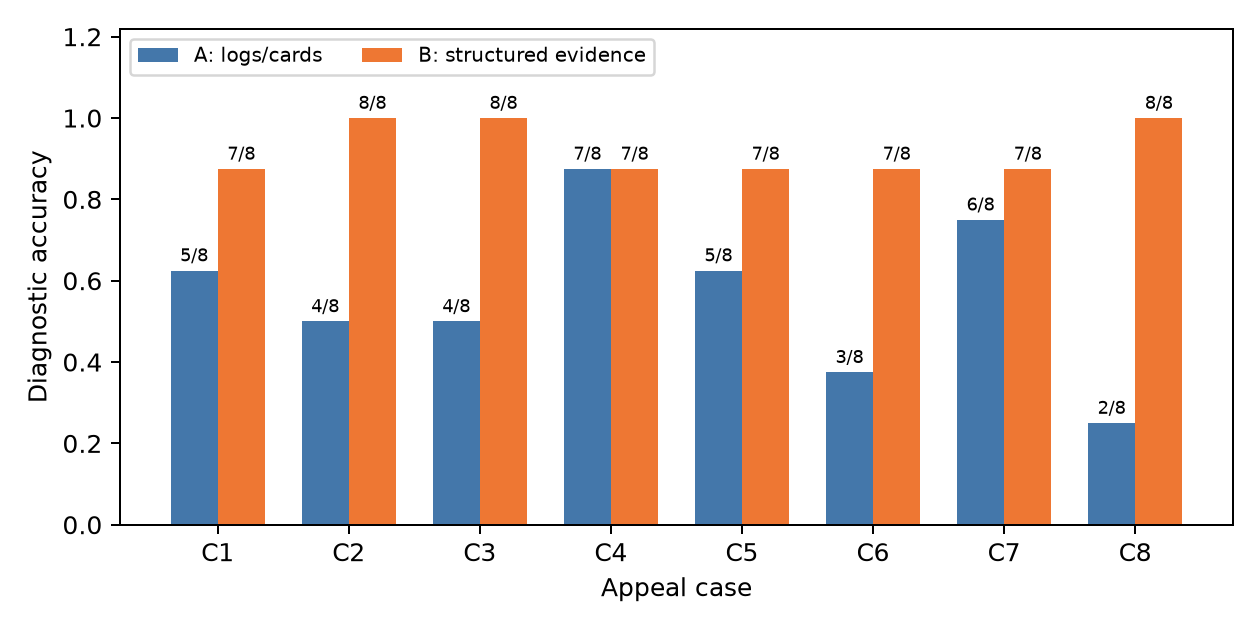
\includegraphics[width=\linewidth]{figures/human_label_accuracy_by_case.png}
\caption{Diagnostic accuracy by case and condition. Labels give exact correct/total counts; all bars have eight responses.}
\Description{Grouped bars compare baseline A and structured-evidence B across eight appeal cases. B equals A in C4 and is higher in the other seven cases. Exact numerators and denominators appear in the adjacent case-count table.}
\label{fig:human-by-case}
\end{figure}

\subsection{Historical states and capacity}
Table~\ref{tab:run-initial} recomputes the historical recipe outcomes and Table~\ref{tab:state-counts} gives exact counts. In the synthetic example $K=100$ but only four cases are eligible and selected; coverage 0.004 is therefore consistent with the capacity ceiling. OULAD similarly selects 69 of a possible 500. Violations were recorded by the historical runner; those records alone do not prove operational escalation.
\begin{table*}[t]
\centering
\small
\caption{PosRate is the selected-set positive outcome rate (legacy Utility@K), not intervention benefit. Historical recipe outcomes, recomputed from emitted states. Entropy thresholds are in bits; VIOL indicates a retrospective ECL violation, not a delivered human review.}
\label{tab:run-initial}
\begin{tabular}{lrrrrrrl}
\toprule
Dataset & $K$ & $\gamma$ & PosRate & Coverage & Abstain & Gap & ECL \\
\midrule
ASSISTments & 1000 & 0.60 & 0.981 & 0.758560 & 0.241440 & 0.00497 & OK \\
OULAD & 500 & 0.60 & 0.174 & 0.010584 & 0.989416 & 0.00192 & VIOL \\
Synthetic & 100 & 0.65 & 1.000 & 0.004000 & 0.996000 & 0.00895 & VIOL \\
\bottomrule
\end{tabular}
\end{table*}

\begin{table*}[t]
\centering
\small
\caption{Exact initial state counts. $K$ is a capacity ceiling, not the realized number selected.}
\label{tab:state-counts}
\begin{tabular}{lrrrrr}
\toprule
Dataset & $n$ & Eligible & Select & Reject & Abstain \\
\midrule
ASSISTments & 105107 & 79730 & 1000 & 78730 & 25377 \\
OULAD & 6519 & 69 & 69 & 0 & 6450 \\
Synthetic & 1000 & 4 & 4 & 0 & 996 \\
\bottomrule
\end{tabular}
\end{table*}


\subsection{Fixed-budget recovery and variable-budget profiles}
Table~\ref{tab:run-sweep} separates full-grid and fixed-budget counts. Table~\ref{tab:recovered} reports achieved metrics of the revised fixed-budget MAS choices. Raising $\gamma$ recovers sample feasibility without retraining, demonstrating a policy-level route to resolve the particular violation. This does not exclude simultaneous model or measurement problems. Table~\ref{tab:policy-profiles} reports separate variable-budget comparisons with the complete profile definitions in Section~\ref{sec:method}. Full precision, group counts, exact grids and candidate IDs are in the structured revision report.
\begin{table}[t]
\centering
\small
\caption{Candidate counts under gap $\leq0.05$ and coverage $\geq0.50$. Full grids vary $K$ and $\gamma$; fixed-budget analyses use only the 16 thresholds at the recipe budget.}
\label{tab:run-sweep}
\begin{tabular}{lrrrrr}
\toprule
Dataset & Full & Feas. & Fixed & Feas. & Pareto \\
\midrule
ASSISTments & 80 & 55 & 16 & 11 & 1 \\
OULAD & 80 & 15 & 16 & 3 & 1 \\
Synthetic & 80 & 12 & 16 & 3 & 1 \\
\bottomrule
\end{tabular}
\end{table}

\begin{table*}[t]
\centering
\small
\caption{Revised MAS selections from the fixed-$K$ feasible Pareto set. All tie tolerances are zero; persistent candidate ID is the final tie-breaker.}
\label{tab:recovered}
\begin{tabular}{lrrrrrrr}
\toprule
Dataset & $K$ & $\gamma$ & Selected & Utility & Gap & Coverage & Abstain \\
\midrule
ASSISTments & 1000 & 0.999 & 1000 & 0.981 & 0.00497 & 0.999448 & 0.000552 \\
OULAD & 500 & 0.999 & 500 & 0.732 & 0.01345 & 0.906427 & 0.093573 \\
Synthetic & 100 & 0.999 & 100 & 1.000 & 0.01697 & 0.933000 & 0.067000 \\
\bottomrule
\end{tabular}
\end{table*}

\begin{table*}[t]
\centering
\small
\caption{Variable-$K$ profiles over the full 80-point grids; these are distinct from fixed-budget recovery. Fairness-first orders gap, utility, abstention; utility-first orders utility, gap, abstention.}
\label{tab:policy-profiles}
\begin{tabular}{llrrrrr}
\toprule
Dataset & Profile & $K$ & $\gamma$ & Utility & Gap & Coverage \\
\midrule
ASSISTments & Fairness-first & 100 & 0.999 & 0.980 & 0.00040 & 0.999448 \\
ASSISTments & Utility-first & 250 & 0.999 & 0.992 & 0.00206 & 0.999448 \\
OULAD & Fairness-first & 50 & 0.999 & 0.800 & 0.00685 & 0.906427 \\
OULAD & Utility-first & 100 & 0.999 & 0.830 & 0.00754 & 0.906427 \\
Synthetic & Fairness-first & 20 & 0.999 & 1.000 & 0.00020 & 0.933000 \\
Synthetic & Utility-first & 20 & 0.999 & 1.000 & 0.00020 & 0.933000 \\
\bottomrule
\end{tabular}
\end{table*}


\subsection{Taxonomy and uncertainty}
Table~\ref{tab:policy-replay} fixes scores, $K$ and $\gamma$ while changing abstention semantics. Utility stays fixed in this example, but automation coverage changes because non-selection can be an automated rejection or a deferral. Treating this as a policy correction requires institutional justification; the numbers alone cannot establish which responsibility assignment is appropriate.
\begin{table*}[t]
\centering
\small
\caption{ASSISTments taxonomy replay with fixed scores, $K=1000$ and $\gamma=0.60$ bits. Changes in automation coverage represent changes in decision responsibility, not demonstrated improvement in student outcomes.}
\label{tab:policy-replay}
\begin{tabular}{lrrrr}
\toprule
Policy & Utility & Coverage & Abstain & Gap \\
\midrule
Global abstention & 0.981 & 0.758560 & 0.241440 & 0.00497 \\
Top-K-only abstention & 0.981 & 1.000000 & 0.000000 & 0.00497 \\
Defer remainder & 0.981 & 0.009514 & 0.990486 & 0.00497 \\
\bottomrule
\end{tabular}
\end{table*}


Table~\ref{tab:uncertainty_proxy_validation} incorporates the previously disconnected numerical validation, recalculated with one entropy convention and average ranks for ties. OULAD has lower entropy/error monotonicity than ASSISTments; the synthetic predictor is poorly calibrated. Temperature scaling can worsen ECE, so we do not claim calibration robustness from preserved rank correlation. The report includes conditional row-bootstrap intervals and group-specific error counts and Wilson intervals across thresholds. Historical interaction packets lack student cluster IDs, so the ASSISTments intervals do not establish cluster-robust uncertainty or field reliability.
\begin{table}[t]
\centering
\small
\caption{Recomputed entropy validation. ECE uses 10 equal-width probability bins including score 1; Spearman uses average ranks for ties. Both baseline and temperature stress use entropy in bits.}
\label{tab:uncertainty_proxy_validation}
\begin{tabular}{lrrrr}
\toprule
Dataset & ECE & $\rho$ & ECE ($T=2$) & $\rho$ ($T=2$) \\
\midrule
ASSISTments & 0.0271 & 0.9789 & 0.0905 & 0.9818 \\
OULAD & 0.0128 & 0.4166 & 0.0703 & 0.4166 \\
Synthetic & 0.2914 & 0.6774 & 0.2398 & 0.6774 \\
\bottomrule
\end{tabular}
\end{table}


\subsection{Artifact checks and appeal scope}
The historical four-point scorecard was populated by constant booleans in the runner, so it is not evidence of independent artifact validation. The revised verifier instead computes integrity and decision-reconstruction checks and tests failures after packet tampering or missing policy content. Fitted-model hashes are separated from configuration hashes; the earlier configuration-only digest is not presented as an immutable trained-model identity.

The appeal pack (Table~\ref{tab:appeal_scenarios}) is a set of study materials. Medical exceptions, changing income, or removing a feature require additional policy inputs or re-scoring and are outside the fixed-score replay contract. Evidence strings in these materials are not execution logs proving that the released engine implements those operations.
\begin{table*}[t]
\centering\small
\caption{Illustrative N=16 study materials, not execution logs. Full Portuguese narratives and A/B evidence strings remain in the eight local case JSONs. The scope column distinguishes fixed-score replay from operations that the engine does not implement.}
\label{tab:appeal_scenarios}
\begin{tabularx}{\textwidth}{lp{.18\textwidth}Xp{.24\textwidth}}
\toprule
Case & Diagnostic category & Evidence illustrated in the instrument & Engine scope \\
\midrule
C1 & Stale input data & Income snapshot and update lineage & Corrected inputs require new inference. \\
C2 & Policy change & Policy versions and effective dates & Fixed-score replay only for supported policy fields. \\
C3 & Normative exception & Medical flag and force-inclusion rule & Exception rule and medical inputs are not implemented. \\
C4 & Capacity constraint & School capacity and revised availability & Global K replay supported; per-school capacity is outside the engine. \\
C5 & Fairness constraint & Group gap and policy cap & Retrospective candidate check; no per-person fairness reranking. \\
C6 & Proxy risk & ZIP-code correlation and feature removal & Proxy audit/removal requires additional analysis or fitting. \\
C7 & Abstention error & Uncertainty value and threshold & Supported score-based abstention reconstruction. \\
C8 & Version mismatch & Declared and executed policy hashes & Content/hash consistency check; no CI/CD system integration. \\
\bottomrule
\end{tabularx}
\end{table*}


\section{Discussion and Limitations}
\label{sec:discussion}
\subsection{Institutional value and responsibility}
An audit trail makes choices inspectable, but does not make the choices legitimate by itself. Constraints are set by actors with authority and incentives; versioning can expose changes but cannot prevent capture or selective compliance \cite{Selbst2019Abstraction,Metcalf2021AIA}. Institutions still need accessible appeal channels, a mandate for policy changes, appropriate staffing and a way to reverse or remedy decisions. A deployment should record who changed a policy, why, who may contest it and how resulting cases are handled.

Automation coverage measures automated outcomes, including rejection. It must not be equated with access to support or students helped. In screening mode the coverage floor can conflict structurally with limited K; increasing automation by relabeling cases changes the division of responsibility between software and staff. Our experiments expose that choice rather than endorse one taxonomy universally.

\subsection{What the evidence establishes}
The strongest evidence is computational: rules can be made explicit, decisions can be replayed on fixed scores, infeasibility can be surfaced, and revised exports can be gated. Sample-level constraints are not population guarantees. Policy selection on the same labelled audit set is exploratory. One historical model and split per dataset do not establish multi-seed predictive stability, comparative state of the art or educational treatment benefit.

The N=16 study is exploratory, uses author-defined standardized scenarios and mixed technical profiles, and has incomplete recruitment and training documentation. Volunteers and consent do not substitute for a formal ethics review, which was not obtained. No causal separation among provenance, structured information and replay is possible in its two conditions. Diagnosis and remediation correctness are perfectly concordant in these responses, so the study provides fewer independent outcome dimensions than its labels might suggest. A prospective study with independent cases, frontline stakeholders and documented institutional review is needed before making field claims.

\subsection{Uncertainty and data limitations}
Predictive entropy is a scalar confidence proxy, not a decomposition of epistemic and aleatoric uncertainty. Calibration and entropy/error correlation do not alone validate the safety of deferral. We therefore provide group-level selective-error summaries and explicitly conditional intervals. ASSISTments uses school-ID parity only to stress the constraint machinery; it does not measure protected-group disparities. OULAD uses binary gender and success labels, leaving wider intersectional and measurement questions unresolved \cite{BakerHawn2022AlgorithmicBiasEducation}.

\subsection{Privacy, integrity and operational boundaries}
Packets must contain the inputs required for the supported rule, with purpose-appropriate access and retention controls. Publishing medical information or raw feature histories is not required by our minimum contract. An institution can keep restricted source evidence behind resolvable references, but missing evidence must be reported rather than treated as replay success. Hashes establish consistency of bytes, not external authenticity or truth. The revised runner's review-required file is not a connected case-management process.

We make no automatic legal-compliance claim. A particular deployment requires jurisdiction-specific institutional review. Instrumented per-case audit cost, staffing capacity, actual access to appeal, independent prospective evaluation and model re-scoring under corrected inputs remain future work. Changing a feature or target creates a new inference or modeling task and must not be described as a policy-only replay.

\section{Conclusion}
\label{sec:conclusion}
We present an artifact-oriented approach to educational decision-system governance: explicit policy, empirical constraints, deterministic feasible-Pareto selection and fixed-score replay. The revision reconciles definitions, identifies the actual outcome-prediction tasks, specifies entropy in bits and capacity ceilings, and separates historical violation reporting from the revised export gate. Computational reports expose policy-dependent feasibility and the consequences of decision taxonomy without implying improved student outcomes.

An exploratory N=16 study supports the complete structured-evidence bundle for standardized appeal diagnosis, with revised statistical reporting and explicit ethical and methodological limits. It does not validate every hypothetical exception, isolate replay from information availability or establish institutional recourse. Future work requires prospective stakeholder evaluation, documented ethical review, independent policy validation, richer uncertainty methods and an instrumented human workflow. Code, exact counts and revision analyses are identified in Appendix~\ref{app:repro}; distribution of participant responses is separate from distribution of aggregate results.

\subsection*{Acknowledgments}
We thank the volunteers and colleagues who contributed to the exploratory evaluation.


\bibliographystyle{ACM-Reference-Format}
\bibliography{references/references}

\begin{table*}[t]
\centering\small
\caption{Focused mechanism comparison with primary sources. This is not an exhaustive capability audit or a measured benchmark of external tools. Entries describe established mechanisms and delimit our own implementation; silence in a source is not treated as proof of an absent feature.}
\label{tab:mechanism-positioning}
\begin{tabularx}{\textwidth}{p{.20\textwidth}XX}
\toprule
Source & Established mechanism & Relationship and limit of this work \\
\midrule
PROV-O \cite{Lebo2013PROVO} & Entities, activities, agents and derivation relations for provenance interchange. & Our decision-packet contract is domain-specific; no implemented PROV-O interchange is claimed. \\
ModelDB \cite{Vartak2016ModelDB} & Model/pipeline history, metadata and metric tracking. & Tracking/versioning itself is established; our evaluated target is the decision contract on fixed scores. \\
Ormenisan et al. \cite{Ormenisan2020TimeTravel} & Change capture and data versions for pipeline reconstruction/debugging. & Our replay does not reconstruct new inference from corrected features. \\
RFC 9162 \cite{Laurie2021RFC9162} & Signed transparency-log structures and inclusion/consistency proofs for certificates. & Local digests and roster checks are weaker: no signed append-only log or independent authenticity. \\
Alfrink et al. \cite{Alfrink2023ContestableAI} & Sociotechnical framework for responsiveness to intervention across the lifecycle. & Fixed-score scrutiny is a bounded enabling mechanism, without an implemented institutional appeal and remedy. \\
\bottomrule
\end{tabularx}
\end{table*}

\section{Code and Data Availability}
\label{app:repro}
\label{app:mechanism-positioning}
The reference repository is \CompassRepoURL. The executable computational snapshot accompanying this manuscript is \path{revisao_artigo/rodada4/pacote_avaliador.zip}, identified by SHA-256 \texttt{108d5ff9f550dec8\allowbreak 82b6691b24ec2b534\allowbreak 0c5515ab3fd550a1\allowbreak 98e32e72e947688}. Its manifest binds source, inputs, protocol, scripts and expected outputs. Commit 227f7fada6f98f44a79a6982dfda26413dcd29ac identifies the published base release, not this snapshot. The embedded paper and present manuscript report the same computational results.

\paragraph{Computational reproduction.}
After extracting the archive, follow its \path{README.md}: use Python 3.12, install \path{requirements.lock}, and run \texttt{python reproduce.py --output-dir actual}. The runner verifies the manifest, regenerates four JSON reports and compares them structurally with the expected outputs, excluding Python patch-version metadata. It runs 20 application tests and checks seven export-contract vectors. The authors executed these checks after extraction; external independent execution remains a separate validation step. The lock records the tested environment; other platforms may require compatibility work.

The source packets are ASSISTments, OULAD and synthetic scored runs from 26 January 2026, all seed 42. The snapshot supplies packet inputs, partition IDs, frozen policies, group counts, expected test metrics and fault results. It does not refit those predictors. Synthetic training fixtures used by application tests are separate from the preserved scored runs. Byte hashes and unsigned local manifests establish consistency within the bundle, not external authenticity against coordinated replacement.

\paragraph{Full-sample and uncertainty analyses.}
The project script \path{revisao_artigo/scripts/recalcular_evidencias.py} generates full-sample candidate tables, group-risk summaries, study aggregates and the diagnostic figure from the preserved inputs. Outputs are in \path{paper_assets/revised/}; structured reports record grids, thresholds, capacities, IDs and counts before display rounding. Fixed-budget and full-grid analyses retain distinct candidate domains. Source and environment inventories accompany these analyses.

\paragraph{Participant data and access restrictions.}
The snapshot excludes participant responses and free text and cannot recompute the human study. That analysis requires locally retained response CSVs and scoring keys. Public materials provide aggregates and methods; generated participants never substitute for restricted responses. Participation and consent records do not establish redistribution rights: individual-data release requires resolution of institutional requirements and sharing permissions. The study analysis and policy-transfer check are retrospective, without prospective preregistration.

The accompanying LaTeX source and computational snapshot have separate inventories. Table~\ref{tab:mechanism-positioning} compares the implemented mechanisms with established approaches and identifies their limits.
 % reproducibility and artifact release
\section{Implementation and Evidence Inventory}
\label{app:implementation}
Preserved scored runs supply metrics, metadata, decision briefs and case packets for each dataset. Policy analyses reuse these scores for sweeps, taxonomy replay and retrospective selection/test evaluation. The schema 2.0 application and synthetic fixtures test evidence verification and export permission. The human study uses separate responses and scenarios; participant data are excluded from the snapshot.

The application source is included under \path{application/} in the snapshot identified in Appendix~\ref{app:repro}. Runs persist policy content, a dataset-manifest copy, fitted-model bytes, separate configuration/model hashes, source-file hashes, selection reports, candidate packets, computed evidence checks and an export gate. A Git HEAD alone does not identify uncommitted source changes. Model snapshots are hashed as opaque bytes; verifying integrity does not require loading serialized code.

The gate permits export after verification and feasibility checks. Infeasibility or insufficient evidence retains candidate metrics and produces a review-required record, without authorized export or delivery to a human queue. Legacy decisions and violation records predate the schema 2.0 guarantees.

The evaluation covers fixed-score policies and the verification contract. Predictive-baseline comparisons, multi-seed modeling, field deployment and individually timed appeal costs remain unevaluated.

\section{Prospective Early-Warning Blueprint: Not Evaluated Here}
\label{app:replication}
A future dropout-prevention use would define a risk-positive outcome, such as Fail/Withdrawn, an intervention horizon, features available before that horizon, and ranking aligned to that objective. It would also require temporal and student-aware splits, label audits and institutionally justified sensitive attributes. These choices differ from the implemented OULAD success target and descending success-score ranking. The current utility values must not be reused as evidence for this proposed task.

Likewise, interaction correctness in ASSISTments is not equivalent to a per-student need-for-support label. Aggregating interactions, selecting an eligible population, specifying the treatment and measuring actual benefit require a separate evaluation. Changing the target or removing features can require retraining; changing an input value requires new inference. Neither operation is a fixed-score policy replay.

\section{Datasets and Implemented Tasks}
\label{app:datasets}
\subsection{ASSISTments}
The 2009--2010 Skill Builder release provides student--problem interactions \cite{Feng2009ASSISTments}. The implemented target is response correctness (positive=1). School-ID parity is a synthetic group for testing constraints, not a demographic or protected attribute.

The processor reads the CSV with a deterministic encoding fallback, replaces decoding errors and skips malformed lines. Numeric missing values are filled with zero, including skill and response-time fields; the implementation does not drop rows for those missing fields. Correctness is coerced to an integer and clipped to zero/one; missing labels become zero. These choices can affect measurement validity and should be audited before deployment.

Features include bounded attempt and hint counts, log-transformed response and overlap times, practice opportunity, an original-item indicator, skill-ID remainder, and fixed one-hot categories for tutor mode, answer type and task type. School ID itself is excluded from the feature vector, but that does not establish absence of proxies.

The runner applies a seed-42 shuffled row split (80/20); the audited output has 105107 cases. Features can describe the interaction being predicted. This is not a temporally validated early-warning task. The historical packets lack student-cluster IDs, so neither split independence nor cluster-robust intervals are established.

\subsection{OULAD}
OULAD provides anonymized student/course information \cite{Kuzilek2017OULAD}. The processor uses the student-information table. Positive means Pass or Distinction; Fail and Withdrawn are negative. Gender F/M defines the binary audit group, with other or missing gender excluded.

Categorical inputs are module, presentation, region, education, deprivation band, age band and disability; numerical inputs are previous attempts and studied credits. Gender and final outcome are excluded from the score features. This is a success-prediction benchmark; it does not use a validated early-intervention time window or estimate treatment benefit. The shuffled 80/20 row split yields 6519 audited cases. Repeated student/course records are not claimed to be separated by student.

\subsection{Synthetic}
The synthetic audit has 1000 held-out cases and a binary generated group. Its purpose is to exercise capacity, abstention, infeasibility and evidence checks under a controlled label process. It is not evidence of field validity. Recipe inputs, hashes and exact group counts are included in the computational revision report.

\section{Artifact Contract and Replay Protocol}
\label{app:artifact-schema}
\subsection{Minimum fixed-score contract}
Schema 2.0 records a persistent case ID, finite score, entropy in bits, clipping convention, decision state, supported replay scope, policy reference/hash, dataset-manifest hash, fitted-model hash and packet hash. Policy content records capacity, score direction, allocation/screening mode, global/Top-$K$-only abstention, threshold/unit and selection criteria/tolerances. Hashes alone are not substitutes for accessible policy content. Labels and audit groups are evaluation fields, separate from decision inputs.

Historical packets have a smaller unversioned schema. Their entropy is checked against the known bit-based implementation before reanalysis; a legacy configuration digest is not described as a fitted-model digest. The revision does not retroactively claim that old packets implemented schema 2.0.

\subsection{Reconstruction and validation}
Replay reads the same fixed scores and case IDs, applies the declared rule and compares every emitted state with the original. The revised verifier additionally checks content hashes, schema/unit fields, policy availability, manifest bytes and model-snapshot bytes. Missing, altered or incompatible evidence causes failure, not a perfect score by default. Tests include score ties, reordered inputs, boundary thresholds, empty feasible sets and corrupted packets.

\subsection{Scope of appeal materials}
Medical-force-inclusion rules require the applicable rule, its version, the relevant flag and exception precedence. These are absent from the minimum score-based contract; no executed medical-exception replay is claimed. Likewise, income corrections or feature removal require updated inputs and re-scoring, possibly retraining. The study's evidence strings are scenario materials rather than logs proving these operations were executed. Restricted evidence may remain outside public bundles, but its availability and access conditions must be documented.

\subsection{Uncertainty analysis}
\label{app:uncertainty}
ECE uses ten equal-width probability bins, including probability one in the final bin. Spearman entropy/absolute-error correlation uses average ranks for ties. Temperature stress uses logits scaled by $T\in\{0.5,2\}$ and recomputes entropy in bits. Conditional percentile intervals use 200 row-bootstrap replicates, seed 42. Per-group selective risk is the binary classification error among entropy-eligible cases, not precision among Top-$K$ selections; reports give error counts, denominators and descriptive Wilson intervals. Interaction packets do not preserve student cluster IDs, so these row-based intervals do not establish cluster-robust population uncertainty.
 % artifact schema + replay protocol

\end{document}
